\section{ICE}

% \begin{frame}[c]{Iterative Correction and Eigenvector decomposition}
%     \Large
%     Algorithm as described in \cite{imakaev2012iterative}.
% \end{frame}


\begin{frame}[c]{ICE as described in Imakaev et al. 2012 \cite{imakaev2012iterative}}
    \Large
    \begin{itemize}[<+(1)->]
        \item $O_{ij}$: raw data
        \item $T_{ij}$: relative contact probabilities
        \item $W_{ij}$: working copy of $O_{ij}$, becoming $T_{ij}$
        \item $S_i$: sum of row $i$ of $W_{ij}$
        \item $B_i, B_j$: cumulative biases
    \end{itemize}
\end{frame}

\begin{frame}[c]{ICE as described in Imakaev et al. 2012 \cite{imakaev2012iterative}}
    \Large
    Goal: Obtain $B$ and $T_{ij}$. \\ \pause Do this by explicitly solving:
    \begin{equation} \label{eq:1}
    O_{ij} = B_i B_j T_{ij}
    \end{equation}
    \begin{equation} \label{eq:2}
    \sum^N_{i=1, |i-j|>1} T_{ij} = 1
    \end{equation}
\end{frame}

\begin{frame}[c]{ICE as described in Imakaev et al. 2012 \cite{imakaev2012iterative}}

    \[
    T_{ij} =
      \begin{bmatrix}
          \tikzmark{topm}{d} & \tikzmark{topr}{d_{+1}} & \tikzmark{suml}{t_{1,3}} & \dots & \dots & \tikzmark{sumr}{t_{1,n}} \\
          \tikzmark{topl}{d_{-1}} & d & d_{+1} & \dots & \dots & t_{2,n} \\
          \vdots & \ddots & \ddots & \ddots & & \vdots \\
          \tikzmark{sl}{\vdots} & \tikzmark{sr}{} & \ddots & \ddots & \ddots & \tikzmark{so}{\vdots} \\
          t_{n-1,1} & \dots & \dots & d_{-1} & d & \tikzmark{lowr}{d_{+1}} \\
          t_{n,1} & \dots & \dots & t_{n,n-2} & \tikzmark{lowl}{d_{-1}} & \tikzmark{lowm}{d}
      \end{bmatrix}
    \]

    \[
    \sum^N_{i=1, |i-j|>1} T_{ij} = 1
    \]

    \only<1>{
    \begin{tikzpicture}[overlay,remember picture]
         \draw[orange,opacity=.4,line width=5mm,line cap=round] (topm.190) -- (sumr.center);
         \draw[blue,opacity=.4,line width=5mm,line cap=round] (sl.210) -- (so.330);
    \end{tikzpicture}
    }

    \pause
    \pause

    \begin{tikzpicture}[overlay,remember picture]
         \draw[opacity=.4,line width=16mm,line cap=round] (topm.315) -- (lowm.150);
    \end{tikzpicture}

    \pause

    \begin{tikzpicture}[overlay,remember picture]
         \draw[orange,opacity=.4,line width=5mm,line cap=round] (suml.center) -- (sumr.center);
         \draw[blue,opacity=.4,line width=5mm,line cap=round] (sl.210) -- (sr.30);
         \draw[blue,opacity=.4,line width=5mm,line cap=round] (so.210) -- (so.330);
    \end{tikzpicture}
\end{frame}

% from: https://tex.stackexchange.com/questions/234989/coloring-the-diagonal-of-a-matrix
% \begin{frame}[c]{ICE as described in Imakaev et al. 2012 \cite{imakaev2012iterative}}
%     \[
%     \begin{bmatrix}
%       \tikzmark{top}{1} & \tikzmark{top2}{1} & 0 \\
%       0 & 1 & \tikzmark{bottom2}{1} \\
%       \tikzmark{end}{1} & 0 & \tikzmark{bottom}{1}\\
%     \end{bmatrix}
%     \]
%
%     \begin{tikzpicture}[overlay,remember picture]
%          \draw[opacity=.4,line width=3mm,line cap=round] (top.center) -- (bottom.center);
%          \draw[opacity=.4,line width=3mm,line cap=round] (top2.center) -- (bottom2.center);
%          \draw[opacity=.4,line width=3mm,line cap=round] (end.center) -- (end.center);
%     \end{tikzpicture}
% \end{frame}


\begin{frame}[c]{ICE as described in Imakaev et al. 2012 \cite{imakaev2012iterative}}
    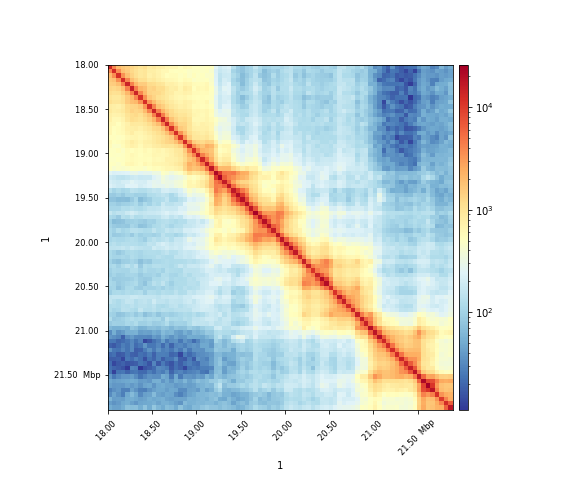
\includegraphics[scale=0.5, trim=50 45 50 30,clip]{c_50kb}
\end{frame}

\begin{frame}[c]{ICE as described in Imakaev et al. 2012 \cite{imakaev2012iterative}}
    \Large
    Each iteration, compute:
    \pause
    \onslide<2->{
    \begin{equation}\label{eq:3}
        S_i = \sum_j W_{ij}
    \end{equation}
    \begin{equation}\label{eq:4}
        \Delta B_i = S_i / mean(S)
    \end{equation}
    }
    \vspace*{-\baselineskip}
    \onslide<3>{
    \begin{equation}\label{eq:5}
        W_{ij} = W_{ij} / \Delta B_i \Delta B_j
    \end{equation}
    \begin{equation}\label{eq:6}
        B_i = B_i \cdot \Delta B_i
    \end{equation}
    }
\end{frame}

% Introduce the ICE algorithms based on graphics / Formulas






